\section{Optimization proposal}
As said in the previous section, the idea is to add a second level of parallelism to apply de Dynamic Load Balancing (DLB) library. This library dynamically lends the node resources of an idle process. For the shared-memory programming model, we choose OmpSs.

\subsection{Concepts}

\subsubsection{OmpSs}
OmpSs\cite{ompss} is a programming model developed at BSC, similarly to OpenMP, is a shared memory programming model based on tasks. It is also used as a forerunner to OpenMP, meaning some proposals and directives are later implemented at OpenMP.


The primary motivation for using OmpSs rather than OpenMP the standard in the HPC community is that OmpSs is better integrated with DLB.

\subsubsection{Dynamic Load Balancing library}
The DLB library\cite{dlb} is a collection of tools aimed to improve and track the performance of parallel applications. 

As we mentioned before DLB can lend unused resources to processes with more load. This mechanism is named "Lend when idle" (LeWI); it intercepts the MPI calls that stall the processes and dynamically lends the threads to other MPI processes within the node which are computing. Figures \ref{nolewiex} and \ref{lewiex} show a comparison between the same execution with 2 MPI processes, each running with two threads, with and without LeWI. Overall we can notice that the execution with LeWI enabled reaches the MPI call earlier because MPI 1 lends its cpus to the MPI 2, meaning that this process will run with 4 cpus. Thus it will finish the execution quicker.
\begin{figure}[h]
  \centering
  \begin{subfigure}{0.4\textwidth}
    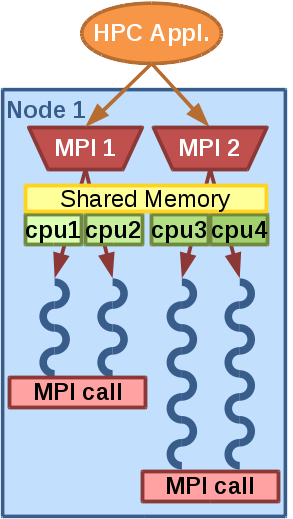
\includegraphics[width=0.8\linewidth]{graphics/dlb_example_nolewi.png}
    \subcaption{No LeWI}
    \label{nolewiex}
  \end{subfigure}
  \hfill
  \centering
  \begin{subfigure}{0.5\textwidth}
    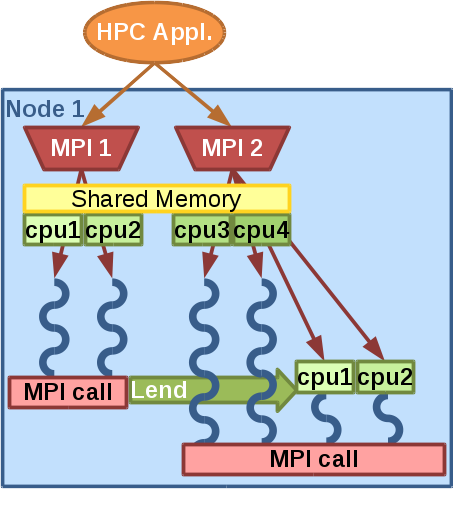
\includegraphics[width=0.8\linewidth]{graphics/dlb_example_lewi.png}
    \subcaption{LeWI}
    \label{lewiex}
  \end{subfigure}
  \caption[LeWI example.]{LeWI example. From DLB website \url{https://pm.bsc.es/dlb}}
  \label{lewiexample}
\end{figure}

\iffalse
\begin{figure}[h]
  \centering
  \begin{subfigure}[b]{1.0\textwidth}
    \begin{tracedraw}{0.7}
      \tracedrawAddToLegend(Useful,blue)
      \tracedrawAddToLegend(Not-useful,red)
      \tracedrawEnableLineName(Process) 
      \tracedrawAddChunk[color=gray, fill=blue](40)
      \tracedrawAddChunk[color=gray, fill=red](60)
      \tracedrawNewLine
      \tracedrawAddChunk[color=gray, fill=blue](80)
      \tracedrawAddChunk[color=gray, fill=red](20)
    \end{tracedraw}
    \caption{No LeWI}
    \label{nolewiex}
  \end{subfigure}
  \hfill
  \centering
  \begin{subfigure}[b]{1.0\textwidth}
    \begin{tracedraw}{0.7}
      \tracedrawAddToLegend(Useful,blue)
      \tracedrawAddToLegend(Not-useful,red)
      \tracedrawAddToLegend(Lend,orange)
      \tracedrawEnableLineName(Process) 
      \tracedrawAddChunk[color=gray, fill=blue](40)
      \tracedrawAddChunk[color=gray, fill=orange](20)
      \tracedrawAddChunk[color=gray, fill=red](40)
      \tracedrawNewLine
      \tracedrawAddChunk[color=gray, fill=blue](60)
      \tracedrawAddChunk[color=gray, fill=red](40)
    \end{tracedraw}
    \caption{LeWI}
    \label{lewiex}
  \end{subfigure}
  \caption[LeWI example.]{LeWI example. Own compilation}
  \label{lewiexample}
\end{figure}
\fi

\subsection{Proposal}
The steps we will follow are:
\begin{itemize}
  \item Hybridize the code, add necessary directives and ensure we don't add any race conditions.
  \item Compile and test the application with OmpSs.
  \item Add DLB support.
  \item Compile and test the application with DLB and OmpSs.
\end{itemize}
